\subsection{Remote procedure calls and *-RPC}
\label{sec:rpc}
Many distributed systems are based on explicit message exchange
between processes. If you see a list of SOA technologies ( provided above, see
\autoref{itm:soa_technologies}) you can find that many of these technologies use
RPC within them. Some of them don't, for example REST described in  previous
section, it uses different resource oriented approach(resources which
the client can consume). Other majority of technologies are message oriented and
use messages for \gls{IPC}. In RPC messages are sent between client and server
to call mathods and receive results. 

\subsubsection{RPC in details}
Remote procedure calls have become a de facto standard for communication
in distributed systems~\cite{tanenbaum07}. The popularity of the model is due to
its apparent simplicity.
This section gives a brief introduction to RPC and the problems in there.

Only one figure is enough to describe RPC(see \autoref{fig:rpc_call}).

% \begin{center}
%  \begin{figure}[h!]
% 	\includegraphics[width=\textwidth]{../images/preliminaries/rpc_diagram.png}
% 	\caption{Principle of RPC between a client and server program }
% 	\label{fig:rpc_call}
%  \end{figure}
% \end{center}
% \includepdf[ angle=90, addtolist={ 1 , figure , {Principle of RPC between a client and server program } , {fig:rpc_call} }
% ]{../images/preliminaries/rpc_diagram.pdf}

% \begin{sidewaysfigure}[h]
%     \includegraphics{../images/preliminaries/rpc_diagram.eps}
%     \caption{Property profile of the diverse library compared to the compound pool.}
%     \label{fig:PropProf}
% \end{sidewaysfigure}


\begin{sidewaysfigure}
\centering
\scalebox{0.4}
{\includegraphics{../images/background/rpc_diagram.png}}
\caption{Principle of RPC between a client and server program}
\label{fig:rpc_call}
\end{sidewaysfigure}


When a process on client machine calls a
procedure on server machine, the calling process on client is suspended, and
execution of the called procedure takes place on server. Information can be
transported from the caller to the callee in the parameters and can come back in the procedure result.
No message passing at all is visible to the programmer. Programmer operates only
with method calls.

The idea behind RPC is to make a remote procedure call look as much as possible
like a local one. In other words, we want RPC to be transparent—the calling
procedure should not be aware that the called procedure is executing on a different
machine or vice versa~\cite{tanenbaum07}. To achieve this transparency special
software modules are used. They are called \textbf{stubs}. The main purpose
of a stub is to handle network messages between client and server. 

Whole RPC call process could be described using words like this: 
\begin{enumerate}
\item The client procedure calls the client stub on the client machine.
\item The client stub builds a message and sends it over the network to remote
machine using local operating system(OS).
\item The remote  OS  receives the message from the network and gives
this message to the server stub. Server stub unpacks the parameters and calls
the server.
\item The server does the work and returns the result to the server stub.
\item The server stub packs result in a message and sends it to client using
network and underlying OS.
\item The client’s OS gives the message to the client stub.The stub unpacks the result and returns to the client.
\item Client receives procedure result and continues his processing.
\end{enumerate}

Modern software tools help to make this process very easy. Here
is the real world example of the small RPC system(written using Python
programming language) that proves this~\cite{xmlrpclib_python_example}:

\begin{listing}[H]
\begin{minted}[frame=lines,
               framesep=2mm]{python}
import xmlrpclib
from SimpleXMLRPCServer import SimpleXMLRPCServer

def is_even(n):
    return n%2 == 0

server = SimpleXMLRPCServer(("example.com", 8000))
print "Listening on port 8000..."
server.register_function(is_even, "is_even")
server.serve_forever()
\end{minted}
\caption{RPC server example (Python and xmlrpclib)}
\label{lst:rpc_server_python_example}
\end{listing}

Code is quite verbose\footnote{Python programming language has its own
philosophy, called The Zen of Python. It has some statements how software
should be designed. Two statements in the Zen of Python that are related to
this example are: \begin{quote}\textit{Simple is better than
complex.}\end{quote}  and \begin{quote}\textit{Readability counts.}\end{quote}}
and people, who are not familiar with Python, could understand it.
You create a server using the special RPC server implementation from
\textit{xmlrpclib} library. You specify a remote host and a port number in a
object constructor. When server object is created you need to specify remote
methods, which may be executed. Example above uses small even check method.
Server registers the methods and starts to wait for incoming calls.

Client implementation for the corresponding server looks like:
\begin{listing}[H]
\begin{minted}[frame=lines,
               framesep=2mm]{python}
import xmlrpclib

proxy = xmlrpclib.ServerProxy("http://example.com:8000/")
print "3 is even: %s" % str(proxy.is_even(3))
print "100 is even: %s" % str(proxy.is_even(100))
\end{minted}
\caption{RPC client example (Python and xmlrpclib)}
\label{lst:rpc_client_python_example}
\end{listing}

Actually, it is more shorter and simpler than server code. You just specify a
remote server object and receive a proxy object. Then you can use this proxy like a usual
local object. This creates an illusion that you are not going anywhere for the
result and working with a usual objects in the code. Proxy object may be passed
as a parameter to a function and be used in that function without knowledge
where it was came from.


This idea is simple and elegant, but there are exist some problems. First of
all, calling and called procedures run on different machines and are executed in
different address spaces, which introduce additional complexity in passing
parameters and results between client and server.
Finally, both machines can independently crash, therefore special error
handling mechanism is required. System developers must deal with such failures
without knowing about remote procedure was actually invoked or not.

As long as the client and server machines are identical and all the parameters
and results are scalar types, such as integers, characters, and Booleans, this model
works fine. 
However, in a large distributed system, it is common that multiple
machine types are present.
Each machine often has its own representation for
numbers, characters, and other data items~\cite{tanenbaum07}.

There are several representations of character data used in computer systems:
one byte characters(ASCII\footnote{ American Standard Code for Information
Interchange}, EBCDIC\footnote{Extended Binary Coded Decimal Interchange Code
(from IBM)}), multibyte characters( UTF-8, UTF-8, UTF-32\footnote{Universal
Character Set Transformation Format},  ) and characters in different
encodings(all tree character encodings are used for cyrillic symbols: 
Windows-1251, Code page 855, ISO/IEC 8859-5). Each RPC client and server should
agree about character encoding they will use.

In addition to that, problems can occur with the representation of integers
(sign-and-magnitude method, one’s complement, two’s complement) and
real data types( floating-point, fixed-point, binary-coded decimal and single
precision, half precision, double precision). Some machines have different
endianness\footnote{The terms little-endian and big-endian refer to the way in which a word of data is stored into sequential bytes of
memory. The first byte of a sequence may store either the least significant byte of a word (little-endian) or the most
significant byte of a word (big-endian). Endianness refers to how bytes and
16-bit half-words map to 32-bit words in the system memory. \cite{arm_endian}}.
If two different machines, one little-endian and other big-endian, are
communicating to each other, they should use common endianness, otherwise they
will accept bytes in wrong order and data will be invalid.

This was a description of primitive data types in RPC so far, but client and
server not always send primitive data types to each other. There could also be a
complex data structures, that contains several primitives like characters,
numbers or just raw bytes. Client and server should be aware of structure of
messages they send and receive. Usually these structures are specified by
Interface Definition Language(IDL).
IDL is a  is a specification language used to describe a software component's interface.
IDLs describe an interface in a language-independent way, enabling
communication between software components that do not share same language and
platform.
An interface is firstly specified in an IDL and then compiled into a
client stub and a server stub. RPC-based middleware systems
offer an IDL to support application development~\cite{tanenbaum07}.

In most cases communication scheme is well known and some standard
message protocol is used. Previous example of RPC system, that was written using
Python programming language, used XML-RPC protocol. XML-RPC defines XML data
types that are used in RPC messages. There are several alternative common used
schemes, that provide similar functionality. They all could be divided into
two groups: platform and programming language dependent and systems that  
can be used in multiplatform and multilanguage environment. XML-RPC belongs to
second group, the similar technologies are JSON-RPC, SOAP and CORBA.
Actually, most RPC implementations in the first group do not require any special
harware. They are programming language dependent and may be used with
the assumption, that components in the system are written using that specific
language. Some examples are provided below:
\begin{itemize}
  \item Java Remote Method Invocation
  \item Pyro object-oriented form of RPC for Python.
  \item Windows Communication Foundation ( .NET framework)
  \item \ldots   
\end{itemize} 
Most of these programming languages have multiplatform implementations and RPC
system may be built using various hardware.

JSON-RPC version 2.0 will be used in this work as primary RPC solution in the implementation of embedded client-server architecture. 
It is based on \gls{JSON} object serialization (see \ref{sec:json_description} section to see information about JSON or visit \url{http://www.json.org/})
and uses JSON format for  transferring messages between client and the server.

JSON-RPC is a lightweight RPC solution that is designed to be simple ~\cite{jsonrpc_spec}.
It defines how client and server should communicate between each other. 
To make a RPC call client needs to send Request object, server need to response with a Response object.

The specification ~\cite{jsonrpc_spec} defines Request object like a stucture with following members:
\begin{itemize}
\item \textbf{jsonrpc} -- A String specifying the version of the JSON-RPC protocol. This must be exactly "2.0".
\item \textbf{method} -- A String containing the name of the method to be invoked.
\item \textbf{params} -- A Structured value that holds the parameter values to be used during the invocation of the method. This member may be omitted.
\item \textbf{id} --  An identifier established by the Client that must contain a String, Number, or NULL value if included. If it is not included the request is assumed to be a notification. 
\end{itemize}

A Notification is a Request object without an "id" member.
A Request object that is a Notification means the Client's lack of interest in the corresponding Response object. 
The Server must not reply to a Notification.

Response object is a JSON object with similar to Request members:

\begin{itemize}
\item \textbf{jsonrpc} -- Has the same meaning as in Request object

\item \textbf{result} --  This member is required on success. It must not exist if there was an error in method invocation.
	This member returns a method result value. It might be complex JSON object. 
\item \textbf{error} --  This member is required on error. This should be a defined object (see below)   

\item \textbf{id} --  Identification  of a client. This member value should be the same, which was sent previously by the client. It may be NULL in case of error
 \end{itemize}

 When there is an error in the RPC call, the Response Object must contain the error member with a value that is a Object with the following members:
\begin{itemize}
\item \textbf{code} -- A Number that indicates the error type that occurred.
\item \textbf{message} --  A String providing a short description of the error.
\item \textbf{data} --     A Primitive or Structured value that contains additional information about the error. This may be omitted.
\end{itemize}	

To give a visual information about these objects and data structures listing \ref{lst:jsonrpc_example} contains examples of client server communication.

\begin{listing}[H]
\begin{minted}[frame=lines,
               framesep=2mm]{javascript}
Legend:
--> data sent to Server
<-- data sent to Client

rpc call with positional parameters:
--> {"jsonrpc": "2.0", "method": "subtract", "params": [42, 23], "id": 1}
<-- {"jsonrpc": "2.0", "result": 19, "id": 1}

--> {"jsonrpc": "2.0", "method": "subtract", "params": [23, 42], "id": 2}
<-- {"jsonrpc": "2.0", "result": -19, "id": 2}

rpc call with named parameters:
--> {"jsonrpc": "2.0", "method": "subtract", 
     "params": {"subtrahend": 23, "minuend": 42}, "id": 3}
<-- {"jsonrpc": "2.0", "result": 19, "id": 3}

--> {"jsonrpc": "2.0", "method": "subtract", 
     "params": {"minuend": 42, "subtrahend": 23}, "id": 4}
<-- {"jsonrpc": "2.0", "result": 19, "id": 4}

a Notification:
--> {"jsonrpc": "2.0", "method": "update", "params": [1,2,3,4,5]}
--> {"jsonrpc": "2.0", "method": "foobar"}

rpc call of non-existent method:
--> {"jsonrpc": "2.0", "method": "foobar", "id": "1"}
<-- {"jsonrpc": "2.0", 
     "error": {"code": -32601, "message": "Method not found"}, 
     "id": "1"}

rpc call with invalid JSON:
--> {"jsonrpc": "2.0", "method": "foobar, "params": "bar", "baz]
<-- {"jsonrpc": "2.0", 
     "error": {"code": -32700, "message": "Parse error"}, 
     "id": null}

rpc call with invalid Request object:
--> {"jsonrpc": "2.0", "method": 1, "params": "bar"}
<-- {"jsonrpc": "2.0", 
     "error": {"code": -32600, "message": "Invalid Request"}, 
     "id": null}

\end{minted}
\caption{JSON-RPC examples of client-server communication ~\cite{jsonrpc_spec}}
\label{lst:jsonrpc_example}
\end{listing}                                                                                                             

JSON-RPC is more simple when it is compared with XML-RPC. 
It is more compact and transport independent 
\footnote{XML-RPC specification at
\url{http://xmlrpc.scripting.com/default.html} tells that it uses HTTP as the
main transport}.
\nameref{sec:xml_vs_json} section provides more detailed comparison of JSON and
XML

\subsubsection{RPC summary}
This section described one another possible way of \gls{IPC}. RPC is used in many
distributed systems in obvious or implicit way. It provides mechanism for calling 
subroutines or procedures on another computer or system. 
Communication in RPC is based on message passing.
The Client sends to the server a message containing request for method call.
The Server sends to the client a message with procedure results.
Modern software tools provide ready RPC libraries and application programmer has no need to explicitly reinvent whole RPC system from scratch.
You can build various distributed systems using RPC.
 


